Boundary value problem (BVP) solvers, such as \texttt{bvp4c}, are designed to treat BVPs in time, see \cite{bvp4cPaper1}. Therefore, they are not equipped to deal with BVPs in both space and time. A method has to be developed that circumvents using BVP solvers and uses initial value problem (IVP) solvers instead. This strategy is called multiple shooting and the theoretical derivation of a multiple shooting approach for PDE-constrained optimization problems can be found in \cite{CarraroIndMultipleShooting} and \cite{CarraroDirectIndirectMultipleShooting}.
\\
In this section, the numerical method is described at the different stages of its development. 
The PDE constraint considered has either Dirichlet or Neumann boundary conditions in space. The problem is treated in one and two dimensions. In order to initiate the development of the method, a simpler PDE constrained optimization problem is considered at first. Once the method is established for the simpler problem, the non-local term is added. After that, two dimensional problems are considered.

\subsubsection{One-Dimensional Diffusion} \label{secNumericsOneDDiffusion1}
One of the simplest cases of a PDE-constrained optimization problem is heat control in one dimension. The PDE constraint involved is the forced heat equation, and the PDE-constrained optimisation problem (\ref{sysOptimalHeating1}), derived in Section \ref{secExactSolsDiffusion1}, is used, and the derived optimality system is treated below. 

The first step in solving this optimality system is to substitute the gradient equation into the heat equation for $u$ and rearranging the equations to only have the time derivative on the left-hand side.
This results in a coupled system of PDEs: 
\begin{align}\label{sysOneDimHeatEqunOptisys1}
\partial_t \rho(r,t) &= \partial_{rr}\rho(r,t) + \frac{1}{\beta}p(r,t),\\
\partial_t p(r,t) &= - \partial_{rr} p(r,t) + \rho(r,t) -\hat{\rho}(r,t), \notag \\
\text{Initial } & \text{and  Final-Time Conditions:}\notag\\
\rho(r,0)&=\rho_0(r),\notag\\
p(r,T) &=0,\notag\\
\text{Dirich} &\text{let  Boundary Conditions:}\notag\\
\rho(r,t) &=0,\quad \text{on} \quad \partial \Omega,\notag\\
p(r,t) &=0,\quad \text{on} \quad \partial \Omega,\notag
\end{align}
where $r \in [a,b]$ and $t \in [0,T]$.
This system is considered as a test problem, since exact solutions for $\rho$ and $p$ are known. Therefore, the exact error of the numerical method can be determined at all points in space and time. The derivation of the exact solutions are discussed in Section \ref{secExactSolsDiffusion1}.

The method that is used to solve this system of PDEs is called the shooting method.
The procedure is to first discretize the problem in space, that is to replace the space derivatives with the appropriate Chebyshev differentiation matrices, as defined above. Then the problem reduces to a coupled system of ODEs, which can be solved using an ODE solver, such as the Matlab solver \texttt{ode15s}. The challenge is that the optimality system is a boundary value problem in time, since the adjoint equation has a final time condition in $p$. 
Therefore, the first idea is to create a guess for the initial condition $p_0(r)$, solve the coupled ODE system using this guess, extracting the computed $p$ value at the final time, $p_{co}(T)$ and measuring the error between the computed $p_{co}$ and the exact $p_{ex}$:
\begin{align*}
e= \norm{p_{co}(T) - p_{ex}(T)}.
\end{align*}
The final step in this procedure is to minimize this error by varying $p_0(r)$, using an in-built Matlab optimization routine, such as \texttt{fsolve}.
This is easily implemented in Matlab, see Appendix \ref{ShootingTest1DiffusionLineBlowsUp}.
However, the problem with this approach is that the adjoint equation, written in this form, is not well posed. The solution to this system blows up in finite time, which is caused by the negative diffusion term in the PDE for $p$.\\

Therefore, the adjoint equation has to be rewritten. This is done by rescaling time as
\begin{align*}
\tau=T+t_0-t,
\end{align*}
which causes the adjoint equation to run backwards in time from $T$ to $t_0=0$. This changes the final time condition for $p$ at time $t=T$, $p(T)=0$, into an initial condition at time $\tau =0$, ${p}(0)=0$.
The optimality system is then:
\begin{align} \label{sysOptimDiffAdjBW1}
\partial_t \rho(r,t) &= \partial_{rr} \rho(r,t) + \frac{1}{\beta}{p}(r,t), \\
\partial_t {p}(r,\tau) &=\partial_{rr} {p}(r,\tau) - \rho(r,\tau) +\hat{\rho}(r,\tau), \notag \\
\text{Initial   } & \text{ Conditions:} \notag  \\
 \rho(r,0)&=\rho_0(r),  \quad \text{for} \quad t=0,\notag \\
{p}(r,0) &=0, \quad \text{for} \quad \tau=0,\notag \\
\text{Dirich} &\text{let Boundary Conditions:} \notag \\
\rho(a,t) &=\rho(b,t)=0, \notag \\
{p}(a,\tau) &={p}(b,\tau)=0, \notag 
\end{align} 
where $t \in [t_0,T]$ and $\tau \in [T,t_0]$.
This is now well posed. However, the issue with this rewritten system is that information about $\rho$ at later times is needed to solve the adjoint equation and ${p}$ values for earlier times are needed to solve the state equation, while neither of these information is available. Figure \ref{ShootingMethod1} visualises this problem. The initial conditions for $\rho$ and $p$ are represented as a green and blue dot respectively. Time $t$ is represented by the green arrow, while time $\tau$, the backwards time, is represented by a blue arrow. In order to test whether this approach works, the exact solution for $\rho$ and $q$ can be used, where information is missing. Then the problem is a decoupled system of PDEs, which is straightforward to solve.  


%\begin{figure}[h] 
%		\vspace{-20pt}
%	\centering
%	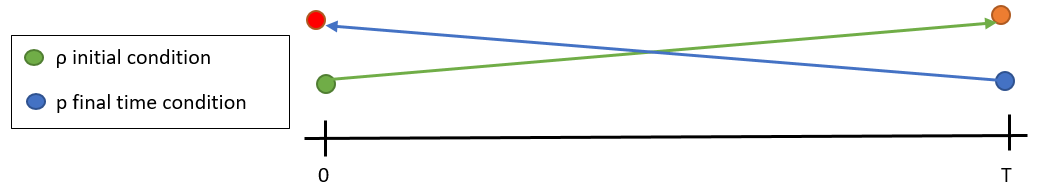
\includegraphics[scale=0.85]{FullSol.png}
%		\vspace{-10pt}
%    \caption{Solving a coupled system of PDEs on $[0,T]$.} 
%    \label{ShootingMethod1}
%    	\vspace{-10pt}
%\end{figure}


In order to replace the missing information, as illustrated above, interpolation is used. Since interpolation using only the endpoints of the interval $[t_0,T]$ would be highly inaccurate, a strategy, called multiple shooting, is exploited in this section. 
The time interval is divided into a number of $n$ subintervals, such that $t_0 < t_1<t_2<...<t_n=T$. The subintervals are denoted by $I_i$, where $i=0,1,...,n-1$. The values for $\rho$ and ${p}$ at these times constitute the initial guess. The discretization of the time interval and initial guesses for $\rho$ and $p$ are illustrated in Figure \ref{ShootingMethod2}. The initial guess can be obtained by different methods, which will be discussed in a later section.

%\begin{figure}[h] 
%	\centering
%	\vspace{-10pt}
%	\includegraphics[scale=0.9]{FullDiscr.png}
%		\vspace{-10pt}
%	\caption{Discretizing the time interval and obtain initial guesses for $\rho$ and $q$.} 
%	\label{ShootingMethod2}
%	\vspace{-10pt}
%\end{figure}

In a first step, these initial guesses are chosen to be the known exact solutions to $\rho$ and ${p}$ at the specified times $t_i$. 
The optimality system (\ref{sysOptimDiffAdjBW1}) is solved on each of the $I_i$, by considering the upper and lower bound of the subinterval, $t_i$ and $t_{i+1}$ instead of the global bounds $t_0$ and $T$. The new backward running time is defined, equivalently to above, as $\tilde\tau =t_{i+1}+t_i-t$, and the system becomes:
\begin{align} \label{sysOptimDiffAdjBW2}
\partial_t \rho(r,t) &= \partial_{rr}\rho(r,t) + \frac{1}{\beta}{p}(r,t), \\
\partial_t {p}(r,\tilde\tau) &= \partial_{rr}{p}(r,\tilde\tau) - \rho(r,\tilde\tau) +\hat{\rho}(r,\tilde\tau), \notag \\
\text{Initial   } & \text{ Conditions:} \notag  \\
\rho(r,t_i)&=\rho_{t_i}, \quad \ \ \text{for} \ \quad t=t_i, \notag \\
{p}(r,t_{i+1}) &=p_{t_{i+1}}, \quad \text{for} \quad \tilde t=t_{i+1}, \notag \\
\text{Dirich} &\text{let  Boundary Conditions:} \notag \\
\rho(a,t) &=\rho(b,t)=0, \notag \\
{p}(a,\tilde\tau) &={p}(b,\tilde\tau)=0, \notag 
\end{align} 
where $t \in I_{i}=[t_i,t_{i+1}]$.
On each subinterval, both $\rho$ and ${p}$ are interpolated between their known values at $t_i$ and $t_{i+1}$, and the result is used to provide $\rho$ at a later time step, to solve the adjoint equation, as well as ${p}$ at an earlier time step, to solve the state equation. 
\newline
\newline
In order to implement the strategy, (\ref{sysOptimDiffAdjBW2}) is evaluated on each time interval $I_i=[t_i,t_{i+1}]$, using interpolation for $\rho$ in the adjoint equation and for $ {p}$ in the state equation to provide the missing information.

%\begin{figure}[h] 
%	\centering
%	\vspace{-10pt}
%	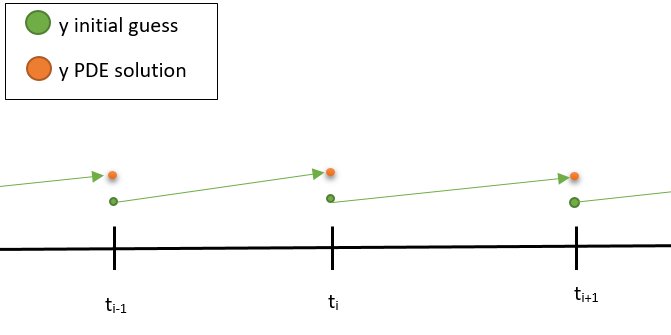
\includegraphics[scale=0.9]{rhoSol.png}
%	\caption{Solution strategy for $\rho$.} 
%	\label{ShootingMethod3}
%\end{figure}
%
%\begin{figure}[h] 
%	\centering
%	\vspace{-20pt}
%	\includegraphics[scale=0.9]{pSol.png}
%	\caption{Solution strategy for $p$.} 
%	\label{ShootingMethod4}
%	\vspace{-10pt}
%\end{figure}

As can be observed in Figure \ref{ShootingMethod3}, the value of $\rho$, taken from the ODE solver, at $t_{i+1}$ is compared to $\rho$ at $t_{i+1}$, which is the initial guess for solving (\ref{sysOptimDiffAdjBW2}) on the next interval $I_{i+1}=[t_{i+1},t_{i+2}]$:
\begin{align}\label{eqnErrorINitoptiguess}
e= \norm{g_{init}-g_{sol}},
\end{align} 
where $g_{init}=(g_1,g_2,...g_n)$ is a vector of initial guesses for $\rho$ on all $n$ time points and $g_{sol}$ is the vector of PDE solutions associated with the initial guesses on all time points.
This provides an error measure of the quality of the set of initial guesses $g_{init}$ for $\rho$. This error calculation is repeated for ${p}$, as illustrated in Figure \ref{ShootingMethod4}. However, since ${p}$ is running backwards in time, the solution to the ODE solver provides the value for ${p}$ at $t_i$, the lower bound on the considered interval $I_i$, which is then compared with the initial guess for ${p}$ for the previous interval $I_{i-1}=[t_{i-1},t_i]$.
Note that for this solution strategy any ODE solver can be used to solve the discretized PDE on each subinterval. Furthermore, while pseudospectral methods are the best method for PDE-constrained optimization problems involving integro-PDE constraints, as discussed in Section \ref{secCompareFEMFDMPDM}, it is in principle possible to use other time or space discretization methods.
\subsubsection{One-Dimensional Diffusion with a Non-Local Term}\label{secOneDDiffusionNonlocalOptim1}
The problem (\ref{sysOptimalHeating1}) is extended by adding a non-local term to the forced heat equation. This non-local term is the two body interaction term that is introduced in Section \ref{secOptimalitySysNonLocal1}.
The one dimensional PDE-constrained optimization problem is:
\begin{align}
&\min_{\rho,u} \quad \frac{1}{2}\norm{\rho- \hat{\rho}}_{L_2}^2 + \frac{\beta}{2} \norm{u}_{L_2}^2,\\
&\text{subject to:}\notag 
\notag \\
&\partial_t \rho - \Delta \rho - u - \nabla \cdot \rho(r) \int_\Omega \nabla V_2(|r-r'|) \rho(r')dr'=0,  \quad \text{in} \quad \Omega,\notag 
\notag \\
&\rho(r,0)=\rho_0(r),\notag 
\notag \\
& \rho(r,t)=0, \quad \text{on} \quad \partial \Omega. \notag 
\end{align}
The first-order optimality system, including the non-local term, is:
\begin{align}\label{sysoptinonlocandheat1D}
\textbf{Adjoint Equation}  \\
\partial_t  p  + \partial_{rr} p + \int_\Omega \bigg(\partial_r  p(r)+\partial_{r'}  p(r')\bigg) \rho(r') \partial_r V_2(|r-r'|) dr' &=(\rho- \hat{\rho})  \quad \text{in} \quad \Omega, \notag \\
p(T) &= 0 \notag\\
p(r,t) &=0 \quad \quad \quad \quad \text{on}\quad \partial\Omega, \notag\\
\textbf{Gradient Equation} \notag \\
\beta u  - \rho  &=0 \quad\quad\quad\quad \text{in} \quad \Omega, \notag \\
\textbf{Forward Problem} \notag \\
\partial_t \rho - \partial_{rr} \rho-u - \partial_r  \rho(r) \int_\Omega \partial_r V_2(|r-r'|) \rho(r')dr' &=0 \quad\quad\quad\quad \text{in} \quad \Omega, \notag \\ 
\rho(r,0)&=\rho_0(r), \notag \\
\rho(r,t) &=0 \quad\quad\quad \quad \text{on} \quad \partial \Omega. \notag
\end{align}
This is directly derived from taking the relevant terms in (\ref{sysFirstOderOptimalityNonLocal1}).
The system that has to be solved on each interval $[t_i,t_{i+1}]$ is, equivalent to (\ref{sysOptimDiffAdjBW2}):
\begin{align*}
\partial_t \rho(r,t) &= \partial_{rr}\rho(r,t) + \frac{1}{\beta}{p}(r,t) + \partial_r  \rho(r,t) \int_\Omega \partial_r V_2(|r-r'|) \rho(r',t)dr', \\
\partial_t {p}(r,\tilde\tau) &= \partial_{rr}{p}(r,\tilde\tau) - \rho(r,\tilde\tau) +\hat{\rho}(r,\tilde\tau) -\int_\Omega \bigg(\partial_r  p(r,\tilde\tau)+\partial_{r'}  p(r',\tilde\tau)\bigg) \rho(r',\tilde\tau) \partial_r V_2(|r-r'|) dr', \notag \\
\text{Initial } & \text{Conditions:} \notag  \\
\rho(r,t_i)&=\rho_{t_i}(r), \quad \quad\text{for} \ \quad t=t_i, \notag \\
{p}(r,t_{i+1}) &=p_{t_{i+1}}(r), \  \quad \text{for} \quad t=t_{i+1}, \notag \\
\text{Dirichl}&\text{et Boundary Conditions:} \notag \\
\rho(a,t) &=\rho(b,t)=0, \notag \\
{p}(a,\tilde\tau) &={p}(b,\tilde\tau)=0, \notag 
\end{align*} 
where $\tilde\tau=t_{i+1} +t_i -t$, as before.
As discussed above, $V_2$ is the force between two particles at positions $r$ and $r'$. It is defined depending on the physical problem involved. For a first numerical test problem, the choice of $V_2$ is a Gaussian:
\begin{align}\label{eqn1Dgaussian}
V_2(x)= \alpha e^{-x^2}.
\end{align}
Then $\partial_r V_2$ satisfies:
\begin{align*}
\partial_r V_2(|r-r'|)= -2\alpha|r-r'| e^{-|r-r'|^2}.
\end{align*}
The specific problem that is solved numerically is:
\begin{align}\label{OptmSysNonloc1alpha}
\partial_t \rho(r,t) &= \partial_{rr}\rho(r,t) + \frac{1}{\beta}{p}(r,t) + \alpha \partial_r  \rho(r,t) \int_\Omega \partial_r  e^{-|r-r'|^2} \rho(r',t)dr', \\
\partial_t {p}(r,\tilde\tau) &= \partial_{rr}{p}(r,\tilde\tau) - \rho(r,\tilde\tau) +\hat{\rho}(r,\tilde\tau) - \alpha\int_\Omega \bigg(\partial_r  p(r,\tilde\tau)+\partial_{r'}  p(r',\tilde\tau)\bigg) \rho(r',\tilde\tau) \partial_r  e^{-|r-r'|^2} dr', \notag \\
\text{Initial } & \text{Conditions:} \notag  \\
\rho(r,0)&=\rho_0(r), \quad \text{for}  \quad t=0, \notag \\
{p}(r,0) &=0,\quad \ \ \quad \text{for} \quad \tilde \tau=0, \notag \\
\notag \\
\text{Dirichl}&\text{et Boundary Conditions:} \notag \\
\rho(a,t) &=\rho(b,t)=0, \notag \\
{p}(a,\tilde\tau) &={p}(b,\tilde\tau)=0. \notag 
\end{align} 

 While the solution method is similar to the approach in Section \ref{secNumericsOneDDiffusion1}, there are two key differences. Firstly, quadrature has to be used, employing (\ref{eqnClenCurtQuad}), to evaluate the integral terms in the optimality system. The other difficulty is that no exact solutions exist to this problem because of the complexity of the non-local term. Therefore, the main issue in solving (\ref{OptmSysNonloc1alpha}) is finding an initial guess on the Chebyshev time points $t_i$, which is close enough to the solution of the system, so that convergence to a continuous solution on the whole interval is possible. The initial guess is found by using a technique called continuation.
 \\
The parameter $\alpha$ in (\ref{OptmSysNonloc1alpha}) represents the strength of the contribution of the integral term to the system of PDEs. 
It can be varied to choose the strength of the particle interactions on the PDE solution. If $\alpha_0=0$, there is no particle interaction and the optimality system for the forced heat equation is recovered, compare to (\ref{sysOptimDiffAdjBW2}).
 Since the solution to that problem is known, the idea is to use the exact solution to the problem where $\alpha_0=0$ as an initial guess to the problem where $\alpha_1$ is non-zero but small.
The optimal initial guess for the problem involving $\alpha_1$ is found by multiple shooting and used as an initial guess for the problem with $\alpha_2$, where $\alpha_2>\alpha_1$. This process is repeated iteratively until a certain contribution of the integral term is reached, for example $\alpha=1$. 
\newline
Generally, the step size in $\alpha$ is not determined linearly, but chosen adaptively. This is because some parts of the problems may be easier to solve than others. If the change in $\alpha$ is chosen small, then the optimization function only needs a few iteration to find the optimal initial guess, based on the result of the previous step in $\alpha$. This is because the problem with $\alpha_{i+1}$ is similar to the problem involving $\alpha_i$ and therefore the optimal initial guesses for the two problems are close. The downside of this approach is that the problem has to be re-evaluated for many different values of $\alpha$, which is computationally expensive. If $\alpha_{i+1}$ is chosen to be considerably larger than $\alpha_i$ at each step, the problem has to be solved less times. However, the risk is that the optimal initial guess for the problem with $\alpha_i$ is not a suitable initial guess for the problem with $\alpha_{i+1}$, and that no solution is found.
There are many ways to change $\alpha$ adaptively and it depends greatly on the problem that is to be solved. 

\subsubsection{Two-Dimensional Problems}\label{sec2Dprobsnum1}
The two dimensional version of the PDE constrained optimization problem (\ref{sysOptimalHeating1}) is treated with numerical methods equivalent to the ones used in one-dimensional case, as discussed in Section \ref{secNumericsOneDDiffusion1}. 
The corresponding optimality system is (\ref{sysPotimaltiyheatequn1}).
All the solution methods follow directly from the one-dimensional method presented in Section \ref{secNumericsOneDDiffusion1}. The only difference is that, instead of having a one-dimensional set of spatial Chebyshev points, a two-dimensional Chebyshev grid has to be used, making use of Kronecker products. This has been introduced in Section \ref{secPSMTheory1}.
One of the things to note is that the computational effort in two dimensions is much higher than for one dimensional calculations. This is because instead of $N$ spatial points, $N_1 \times N_2$ spatial points have to be evaluated.

\subsubsection{Two-Dimensional Problems with a Non-Local Term}
Adding a non-local term to (\ref{sysOptimalHeating1}), the PDE-constrained optimization problem becomes:
\begin{align*}
&\min_{\rho,u} \quad \frac{1}{2}\norm{\rho- \hat{\rho}}_{L_2}^2 + \frac{\beta}{2} \norm{u}_{L_2}^2,\\
\\
&\text{subject to:}\\
&\partial_t \rho = \Delta \rho + {u} + \nabla \cdot \int_\Omega \rho(r) \rho(r') \nabla V_2(|r-r'|)dr'  \quad \text{in} \quad \Omega,
\\
&\rho(r,0)=\rho_0(r),
\\
& \rho(r,t)=0, \quad\quad\quad\quad\quad\quad\quad\quad\quad\quad\quad\quad\quad\quad\quad\quad \quad  \text{on} \quad \partial \Omega,
\end{align*}
where $r=(x,y) \in \mathbf{R}^2$.
The corresponding optimality system is:
\begin{align*}
\textbf{Adjoint Equation}  \\
\partial_t p(r,\tau) &= \Delta p(r,\tau) -\rho(r,\tau) +\hat{\rho}(r,\tau)\\
&-\int_\Omega \bigg( \nabla_r p(r,\tau) + \nabla_{r'} p(r',\tau) \bigg) \rho(r',t) \nabla_r V_2(|r-r'|)dr'  \quad\quad\quad   \text{in} \quad \Omega,\\
p(T) &= 0 \notag\\
p(r,t) &=0 \quad \quad \quad  \quad\quad\quad\quad\quad\quad\quad\quad\quad\quad\quad\quad\quad\quad\quad\quad\quad\quad\quad\quad \quad\ \ \ \text{on}\quad \partial\Omega, \notag\\
\textbf{Gradient Equation} \notag \\
\beta u  - \rho  &=0 \quad\quad\quad\quad \quad\quad\quad\quad\quad\quad\quad\quad\quad\quad\quad\quad\quad\quad\quad\quad\quad\quad\quad\quad\quad\text{in} \quad \Omega, \notag \\
\textbf{Forward Problem} \notag \\
\partial_t \rho(r,t) &= \Delta \rho(r,t) + u(r,t)+  \nabla_r \cdot \int_\Omega \rho(r,t) \rho(r',t) \nabla_r V_2(|r-r'|)dr' \quad \ \text{in} \quad \Omega,\\  
\rho(r,0)&=\rho_0(r), \notag \\
\rho(r,t) &=0 \quad\quad\quad \quad\quad\quad\quad\quad\quad\quad\quad\quad\quad\quad\quad\quad\quad \quad\quad\quad\quad\quad\quad\quad \ \ \ \text{on} \quad \partial \Omega, \notag
\end{align*}
compare with the one-dimensional system (\ref{sysoptinonlocandheat1D}).
Equivalently to the one-dimensional particle interaction term, (\ref{eqn1Dgaussian}), $V_2$ is the two-dimensional Gaussian:
\begin{align*}
V_2(x,y)= \alpha e^{-(x^2 +y^2)}.
\end{align*}
When substituting the gradient equation into the state equation, the optimality system becomes:
\begin{align}\label{OptmSysNonloc1alpha2D}
\partial_t \rho(r,t) &= \Delta\rho(r,t) + \frac{1}{\beta}{p}(r,t) + \alpha \nabla_r \cdot  \int_\Omega \nabla_r\bigg(  e^{-|r-r'|^2} \bigg)\rho(r',t)\rho(r,t)dr', \\
\partial_t {p}(r,\tilde\tau) &=\Delta {p}(r,\tilde\tau) - \rho(r,\tilde\tau) +\hat{\rho}(r,\tilde\tau) - \alpha\int_\Omega \bigg(\nabla_r  p(r,\tilde\tau)+\nabla_{r'}  p(r',\tilde\tau)\bigg) \cdot \nabla_r \bigg(  e^{-|r-r'|^2} \bigg)\rho(r',\tilde\tau)  dr', \notag \\
\text{Initial } & \text{Conditions:} \notag  \\
\rho(r,0)&=\rho_0(r), \quad \text{for}  \quad t=0, \notag \\
{p}(r,0) &=0,\quad \ \ \quad \text{for} \quad \tilde \tau=0, \notag \\
\text{Dirichl}&\text{et Boundary Conditions:} \notag \\
\rho(a,t) &=\rho(b,t)=0, \notag \\
{p}(a,\tilde\tau) &={p}(b,\tilde\tau)=0, \notag 
\end{align}
where $\tilde \tau= T+t_0 -t$. 
The method for solving this system, including multiple shooting and continuation, follows exactly from the one-dimensional approach discussed in Section \ref{secOneDDiffusionNonlocalOptim1}.